\PassOptionsToPackage{unicode=true}{hyperref} % options for packages loaded elsewhere
\PassOptionsToPackage{hyphens}{url}
\PassOptionsToPackage{dvipsnames,svgnames*,x11names*}{xcolor}
%
\documentclass[10pt,ignorenonframetext,serif,onlymath]{beamer}
\setbeamertemplate{caption}[numbered]
\setbeamertemplate{caption label separator}{: }
\setbeamercolor{caption name}{fg=normal text.fg}
\beamertemplatenavigationsymbolsempty
\usepackage{lmodern}
\usepackage{amssymb,amsmath}
\usepackage{ifxetex,ifluatex}
\usepackage{fixltx2e} % provides \textsubscript
\ifnum 0\ifxetex 1\fi\ifluatex 1\fi=0 % if pdftex
  \usepackage[T1]{fontenc}
  \usepackage[utf8]{inputenc}
  \usepackage{textcomp} % provides euro and other symbols
\else % if luatex or xelatex
  \usepackage{unicode-math}
  \defaultfontfeatures{Ligatures=TeX,Scale=MatchLowercase}
\fi
% use upquote if available, for straight quotes in verbatim environments
\IfFileExists{upquote.sty}{\usepackage{upquote}}{}
% use microtype if available
\IfFileExists{microtype.sty}{%
\usepackage[]{microtype}
\UseMicrotypeSet[protrusion]{basicmath} % disable protrusion for tt fonts
}{}
\IfFileExists{parskip.sty}{%
\usepackage{parskip}
}{% else
\setlength{\parindent}{0pt}
\setlength{\parskip}{6pt plus 2pt minus 1pt}
}
\usepackage{xcolor}
\usepackage{hyperref}
\hypersetup{
            pdftitle={Sampling with Halton Points on n-Sphere},
            pdfauthor={Wai-Shing~Luk},
            colorlinks=true,
            linkcolor=Maroon,
            citecolor=Blue,
            urlcolor=Blue,
            breaklinks=true}
\urlstyle{same}  % don't use monospace font for urls
\newif\ifbibliography
\usepackage{color}
\usepackage{fancyvrb}
\newcommand{\VerbBar}{|}
\newcommand{\VERB}{\Verb[commandchars=\\\{\}]}
\DefineVerbatimEnvironment{Highlighting}{Verbatim}{commandchars=\\\{\}}
% Add ',fontsize=\small' for more characters per line
\newenvironment{Shaded}{}{}
\newcommand{\AlertTok}[1]{\textcolor[rgb]{1.00,0.00,0.00}{\textbf{#1}}}
\newcommand{\AnnotationTok}[1]{\textcolor[rgb]{0.38,0.63,0.69}{\textbf{\textit{#1}}}}
\newcommand{\AttributeTok}[1]{\textcolor[rgb]{0.49,0.56,0.16}{#1}}
\newcommand{\BaseNTok}[1]{\textcolor[rgb]{0.25,0.63,0.44}{#1}}
\newcommand{\BuiltInTok}[1]{#1}
\newcommand{\CharTok}[1]{\textcolor[rgb]{0.25,0.44,0.63}{#1}}
\newcommand{\CommentTok}[1]{\textcolor[rgb]{0.38,0.63,0.69}{\textit{#1}}}
\newcommand{\CommentVarTok}[1]{\textcolor[rgb]{0.38,0.63,0.69}{\textbf{\textit{#1}}}}
\newcommand{\ConstantTok}[1]{\textcolor[rgb]{0.53,0.00,0.00}{#1}}
\newcommand{\ControlFlowTok}[1]{\textcolor[rgb]{0.00,0.44,0.13}{\textbf{#1}}}
\newcommand{\DataTypeTok}[1]{\textcolor[rgb]{0.56,0.13,0.00}{#1}}
\newcommand{\DecValTok}[1]{\textcolor[rgb]{0.25,0.63,0.44}{#1}}
\newcommand{\DocumentationTok}[1]{\textcolor[rgb]{0.73,0.13,0.13}{\textit{#1}}}
\newcommand{\ErrorTok}[1]{\textcolor[rgb]{1.00,0.00,0.00}{\textbf{#1}}}
\newcommand{\ExtensionTok}[1]{#1}
\newcommand{\FloatTok}[1]{\textcolor[rgb]{0.25,0.63,0.44}{#1}}
\newcommand{\FunctionTok}[1]{\textcolor[rgb]{0.02,0.16,0.49}{#1}}
\newcommand{\ImportTok}[1]{#1}
\newcommand{\InformationTok}[1]{\textcolor[rgb]{0.38,0.63,0.69}{\textbf{\textit{#1}}}}
\newcommand{\KeywordTok}[1]{\textcolor[rgb]{0.00,0.44,0.13}{\textbf{#1}}}
\newcommand{\NormalTok}[1]{#1}
\newcommand{\OperatorTok}[1]{\textcolor[rgb]{0.40,0.40,0.40}{#1}}
\newcommand{\OtherTok}[1]{\textcolor[rgb]{0.00,0.44,0.13}{#1}}
\newcommand{\PreprocessorTok}[1]{\textcolor[rgb]{0.74,0.48,0.00}{#1}}
\newcommand{\RegionMarkerTok}[1]{#1}
\newcommand{\SpecialCharTok}[1]{\textcolor[rgb]{0.25,0.44,0.63}{#1}}
\newcommand{\SpecialStringTok}[1]{\textcolor[rgb]{0.73,0.40,0.53}{#1}}
\newcommand{\StringTok}[1]{\textcolor[rgb]{0.25,0.44,0.63}{#1}}
\newcommand{\VariableTok}[1]{\textcolor[rgb]{0.10,0.09,0.49}{#1}}
\newcommand{\VerbatimStringTok}[1]{\textcolor[rgb]{0.25,0.44,0.63}{#1}}
\newcommand{\WarningTok}[1]{\textcolor[rgb]{0.38,0.63,0.69}{\textbf{\textit{#1}}}}
\usepackage{graphicx,grffile}
\makeatletter
\def\maxwidth{\ifdim\Gin@nat@width>\linewidth\linewidth\else\Gin@nat@width\fi}
\def\maxheight{\ifdim\Gin@nat@height>\textheight\textheight\else\Gin@nat@height\fi}
\makeatother
% Scale images if necessary, so that they will not overflow the page
% margins by default, and it is still possible to overwrite the defaults
% using explicit options in \includegraphics[width, height, ...]{}
\setkeys{Gin}{width=\maxwidth,height=\maxheight,keepaspectratio}
% Prevent slide breaks in the middle of a paragraph:
\widowpenalties 1 10000
\raggedbottom
\setbeamertemplate{part page}{
\centering
\begin{beamercolorbox}[sep=16pt,center]{part title}
  \usebeamerfont{part title}\insertpart\par
\end{beamercolorbox}
}
\setbeamertemplate{section page}{
\centering
\begin{beamercolorbox}[sep=12pt,center]{part title}
  \usebeamerfont{section title}\insertsection\par
\end{beamercolorbox}
}
\setbeamertemplate{subsection page}{
\centering
\begin{beamercolorbox}[sep=8pt,center]{part title}
  \usebeamerfont{subsection title}\insertsubsection\par
\end{beamercolorbox}
}
\AtBeginPart{
  \frame{\partpage}
}
\AtBeginSection{
  \ifbibliography
  \else
    \frame{\sectionpage}
  \fi
}
\AtBeginSubsection{
  \frame{\subsectionpage}
}
\setlength{\emergencystretch}{3em}  % prevent overfull lines
\providecommand{\tightlist}{%
  \setlength{\itemsep}{0pt}\setlength{\parskip}{0pt}}
\setcounter{secnumdepth}{0}

% set default figure placement to htbp
\makeatletter
\def\fps@figure{htbp}
\makeatother

\usetheme{default}
\usepackage{tikz,pgf,pgfplots}
\usetikzlibrary{arrows}
\definecolor{qqqqff}{rgb}{0.,0.,1.}
\newcommand{\columnsbegin}{\begin{columns}}
\newcommand{\columnsend}{\end{columns}}
\newcommand{\col}[1]{\column{#1}}
\pgfdeclareimage[height=0.5cm]{fudan-logo}{fudan-logo.jpg}
\logo{\pgfuseimage{fudan-logo}}

\title{Sampling with Halton Points on n-Sphere}
\author{Wai-Shing~Luk}
\providecommand{\institute}[1]{}
\institute{Fudan University}
\date{\today}

\begin{document}
\frame{\titlepage}

\begin{frame}
\tableofcontents[hideallsubsections]
\end{frame}
\hypertarget{abstract}{%
\section{Abstract}\label{abstract}}

\begin{frame}{Abstract}
\protect\hypertarget{abstract-1}{}

\begin{itemize}
\item
  Sampling on \(n\)-sphere (\(S^n\)) has a wide range of applications,
  such as:

  \begin{itemize}
  \item
    Spherical coding in MIMO wireless communication
  \item
    Multivariate empirical mode decomposition
  \item
    Filter bank design
  \end{itemize}
\item
  We propose a simple yet effective method which:

  \begin{itemize}
  \item
    Utilizes low-discrepancy sequence
  \item
    Contains only 10 lines of MATLAB code in our implementation!
  \item
    Allow incremental generation.
  \end{itemize}
\item
  Numerical results show that the proposed method outperforms the
  randomly generated sequences and other proposed methods.
\end{itemize}

\end{frame}

\hypertarget{motivation-and-applications}{%
\section{Motivation and
Applications}\label{motivation-and-applications}}

\begin{frame}{Problem Formulation}
\protect\hypertarget{problem-formulation}{}

Desirable properties of samples over \(S^n\)

\begin{itemize}
\item
  Uniform
\item
  Deterministic
\item
  Incremental

  \begin{itemize}
  \item
    The uniformity measures are optimized with every new point.
  \item
    Reason: in some applications, it is unknown how many points are
    needed to solve the problem in advance
  \end{itemize}
\end{itemize}

\end{frame}

\begin{frame}{Motivation}
\protect\hypertarget{motivation}{}

\begin{itemize}
\item
  The topic has been well studied for sphere in 3D, i.e. \(n=2\)
\item
  Yet it is still unknown how to generate for \(n > 2\).
\item
  Potential applications (for \(n > 2\)):

  \begin{itemize}
  \item
    Robotic Motion Planning (\(S^3\) and SO(3))~(Yershova et al.
    \protect\hyperlink{ref-yershova2010generating}{2010})
  \item
    Spherical coding in MIMO wireless communication~(Utkovski and
    Lindner \protect\hyperlink{ref-utkovski2006construction}{2006}):

    \begin{itemize}
    \item
      Cookbook for Unitary matrices
    \item
      A code word = a point in \(S^n\)
    \end{itemize}
  \item
    Multivariate empirical mode decomposition~(Rehman and Mandic
    \protect\hyperlink{ref-rehman2010multivariate}{2010})
  \item
    Filter bank design~(Mandic and others
    \protect\hyperlink{ref-mandic2011filter}{2011})
  \end{itemize}
\end{itemize}

\end{frame}

\begin{frame}{Halton Sequence on \(S^n\)}
\protect\hypertarget{halton-sequence-on-sn}{}

\begin{itemize}
\item
  Halton sequence on \(S^2\) has been well studied~(Cui and Freeden
  \protect\hyperlink{ref-cui1997equidistribution}{1997}) by using
  cylindrical coordinates.
\item
  Yet it is still little known for \(S^n\) where \(n>2\).
\item
  Note: The generalization of cylindrical coordinates does NOT work in
  higher dimensions.
\end{itemize}

\end{frame}

\hypertarget{review-of-low-discrepancy-sequence}{%
\section{Review of Low Discrepancy
Sequence}\label{review-of-low-discrepancy-sequence}}

\begin{frame}{Basic: Van der Corput sequence}
\protect\hypertarget{basic-van-der-corput-sequence}{}

\begin{itemize}
\item
  Generate a low discrepancy sequence over \([0,1]\)
\item
  Denote \(\mathrm{vd}(k,b)\) as a Van der Corput sequence of \(k\)
  points, where \(b\) is the base of a prime number.
\item
  MATLAB source code is available at
  \href{http://www.mathworks.com/matlabcentral/fileexchange/15354-generate-a-van-der-corput-sequence}{here}
\end{itemize}

\begin{figure}[hp]
\centering
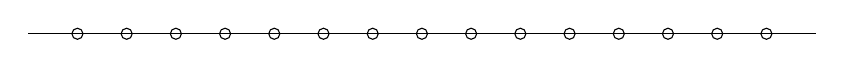
\begin{tikzpicture}[>=latex',line join=bevel]
    %\draw[help lines] (0,0) grid +(10,3);
    \draw (0,1) -- (10,1); \pause
    \draw (5,1) circle (2pt); \pause
    \draw (2.5,1) circle (2pt); \pause
    \draw (7.5,1) circle (2pt); \pause
    \draw (1.25,1) circle (2pt); \pause
    \draw (6.25,1) circle (2pt); \pause
    \draw (3.75,1) circle (2pt); \pause
    \draw (8.75,1) circle (2pt); \pause
    \draw (0.625,1) circle (2pt); \pause
    \draw (5.625,1) circle (2pt); \pause
    \draw (3.125,1) circle (2pt); \pause
    \draw (8.125,1) circle (2pt); \pause
    \draw (1.875,1) circle (2pt); \pause
    \draw (6.875,1) circle (2pt); \pause
    \draw (4.375,1) circle (2pt); \pause
    \draw (9.375,1) circle (2pt);
\end{tikzpicture}

\caption{Example of Van der Corput sequence}%
\label{fig:vdc}
\end{figure}

\end{frame}

\begin{frame}{Halton sequence on \([0,1]\)}
\protect\hypertarget{halton-sequence-on-01}{}

\begin{columns}

\column{0.45\textwidth}

\begin{itemize}
\item
  Halton sequence: using 2 Van der Corput sequences with different
  bases.
\item
  Example: \[[x,y] = [\mathrm{vd}(k,2), \mathrm{vd}(k,3)]\]
\end{itemize}

\column{0.45\textwidth}

\begin{figure}[hp]
\centering
\begin{tikzpicture}[line cap=round,line join=round,>=triangle 45,x=5cm,y=5cm]
    %\begin{tikzpicture}[>=latex',line join=bevel]
    %\clip(-4.3,-2.96) rectangle (11,11);
    \draw (0,0) -- (1,0); 
    \draw (1,0) -- (1,1);
    \draw (1,1) -- (0,1); 
    \draw (0,1) -- (0,0); \pause
    %\draw (     0,      0) circle (2pt); \pause
    \draw (0.5000, 0.3333) circle (2pt); \pause
    \draw (0.2500, 0.6667) circle (2pt); \pause
    \draw (0.7500, 0.1111) circle (2pt); \pause
    \draw (0.1250, 0.4444) circle (2pt); \pause
    \draw (0.6250, 0.7778) circle (2pt); \pause
    \draw (0.3750, 0.2222) circle (2pt); \pause
    \draw (0.8750, 0.5556) circle (2pt); \pause
    \draw (0.0625, 0.8889) circle (2pt); \pause
    \draw (0.5625, 0.0370) circle (2pt); \pause
    \draw (0.3125, 0.3704) circle (2pt); \pause
    \draw (0.8125, 0.7037) circle (2pt); \pause
    \draw (0.1875, 0.1481) circle (2pt); \pause
    \draw (0.6875, 0.4815) circle (2pt); \pause
    \draw (0.4375, 0.8148) circle (2pt); \pause
    \draw (0.9375, 0.2593) circle (2pt); \pause
    \draw (0.0313, 0.5926) circle (2pt); \pause
    \draw (0.5313, 0.9259) circle (2pt); \pause
    \draw (0.2813, 0.0741) circle (2pt); \pause
    \draw (0.7813, 0.4074) circle (2pt); \pause
    \draw (0.1563, 0.7407) circle (2pt); \pause
    \draw (0.6563, 0.1852) circle (2pt); \pause
    \draw (0.4063, 0.5185) circle (2pt); \pause
    \draw (0.9063, 0.8519) circle (2pt); \pause
    \draw (0.0938, 0.2963) circle (2pt); 
\end{tikzpicture}

\caption{Example of Halton sequnce}%
\label{fig:halton}
\end{figure}

\end{columns}

\end{frame}

\begin{frame}{Halton sequence on \([0,1]^n\)}
\protect\hypertarget{halton-sequence-on-01n}{}

\begin{itemize}
\item
  Generally we can generate Halton sequence in a unit hypercube
  \([0,1]^n\):

  \[[x_1, x_2, \ldots, x_n] = [\mathrm{vd}(k,b_1), \mathrm{vd}(k,b_2), \ldots, \mathrm{vd}(k,b_n)]\]
\item
  A wide range of applications on Quasi-Monte Carlo Methods (QMC).
\end{itemize}

\end{frame}

\begin{frame}{Unit Circle \(S^1\)}
\protect\hypertarget{unit-circle-s1}{}

\begin{columns}

\column{0.6\textwidth}

Can be generated by mapping the Van der Corput sequence to \([0, 2\pi]\)

\begin{itemize}
\item
  \(\theta = 2\pi \cdot \mathrm{vd}(k,b)\)
\item
  \([x, y] = [\cos\theta, \sin\theta]\)
\end{itemize}

\column{0.4\textwidth}

\begin{figure}[hp]
\centering
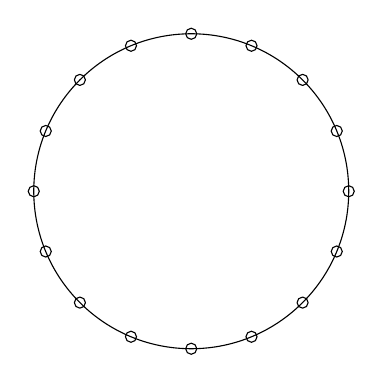
\begin{tikzpicture}[line cap=round,line join=round,>=triangle 45,x=2cm,y=2cm]
   \draw (0,0) circle (1); \pause
   \draw ( 1.0000,       0) circle (2pt); \pause
   \draw (-1.0000,  0.0000) circle (2pt); \pause
   \draw ( 0.0000,  1.0000) circle (2pt); \pause
   \draw (-0.0000, -1.0000) circle (2pt); \pause
   \draw ( 0.7071,  0.7071) circle (2pt); \pause
   \draw (-0.7071, -0.7071) circle (2pt); \pause
   \draw (-0.7071,  0.7071) circle (2pt); \pause
   \draw ( 0.7071, -0.7071) circle (2pt); \pause
   \draw ( 0.9239,  0.3827) circle (2pt); \pause
   \draw (-0.9239, -0.3827) circle (2pt); \pause
   \draw (-0.3827,  0.9239) circle (2pt); \pause
   \draw ( 0.3827, -0.9239) circle (2pt); \pause
   \draw ( 0.3827,  0.9239) circle (2pt); \pause
   \draw (-0.3827, -0.9239) circle (2pt); \pause
   \draw (-0.9239,  0.3827) circle (2pt); \pause
   \draw ( 0.9239, -0.3827) circle (2pt);
\end{tikzpicture}

\caption{Sequnce mapping to a unit circle}%
\label{fig:circle}
\end{figure}

\end{columns}

\end{frame}

\begin{frame}{Unit Sphere \(S^2\)}
\protect\hypertarget{unit-sphere-s2}{}

\begin{columns}

\column{0.6\textwidth}

Has been applied for computer graphic applications~(Wong, Luk, and Heng
\protect\hyperlink{ref-wong1997sampling}{1997})

\begin{itemize}
\item
  \([z, x, y]\)\\
  = \([\cos\theta, \sin\theta\cos\varphi, \sin\theta\sin\varphi]\)\\
  = \([z, \sqrt{1-z^2}\cos\varphi, \sqrt{1-z^2}\sin\varphi]\)
\item
  \(\varphi = 2\pi\cdot\mathrm{vd}(k,b_1)\) \% map to \([0,2\pi]\)
\item
  \(z = 2\cdot\mathrm{vd}(k,b_2) - 1\) \% map to \([-1,1]\)
\end{itemize}

\column{0.4\textwidth}

\begin{figure}
\centering
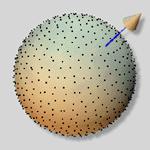
\includegraphics[width=0.8\textwidth,height=\textheight]{thammer.png}
\caption{image}
\end{figure}

\end{columns}

\end{frame}

\begin{frame}{Sphere \(S^n\) and SO(3)}
\protect\hypertarget{sub:sphere_s_n_and_so_3_}{}

\begin{itemize}
\item
  Deterministic point sets

  \begin{itemize}
  \tightlist
  \item
    Optimal grid point sets for \(S^3\), SO(3) {[}Lubotzky, Phillips,
    Sarnak 86{]} {[}Mitchell 07{]}
  \end{itemize}
\item
  No Halton sequences so far to the best of our knowledge
\end{itemize}

\end{frame}

\hypertarget{our-approach}{%
\section{Our approach}\label{our-approach}}

\begin{frame}{SO(3) or \(S^3\) Hopf Coordinates}
\protect\hypertarget{so3-or-s3-hopf-coordinates}{}

\begin{columns}

\column{0.6\textwidth}

\begin{itemize}
\item
  Hopf coordinates (cf.~(Yershova et al.
  \protect\hyperlink{ref-yershova2010generating}{2010}))

  \begin{itemize}
  \item
    \(x_1 = \cos(\theta/2) \cos(\psi/2)\)
  \item
    \(x_2 = \cos(\theta/2) \sin(\psi/2)\)
  \item
    \(x_3 = \sin(\theta/2) \cos(\varphi + \psi/2)\)
  \item
    \(x_4 = \sin(\theta/2) \sin(\varphi + \psi/2)\)
  \end{itemize}
\item
  \(S^3\) is a principal circle bundle over the \(S^2\)
\end{itemize}

\column{0.4\textwidth}

\begin{figure}
\centering
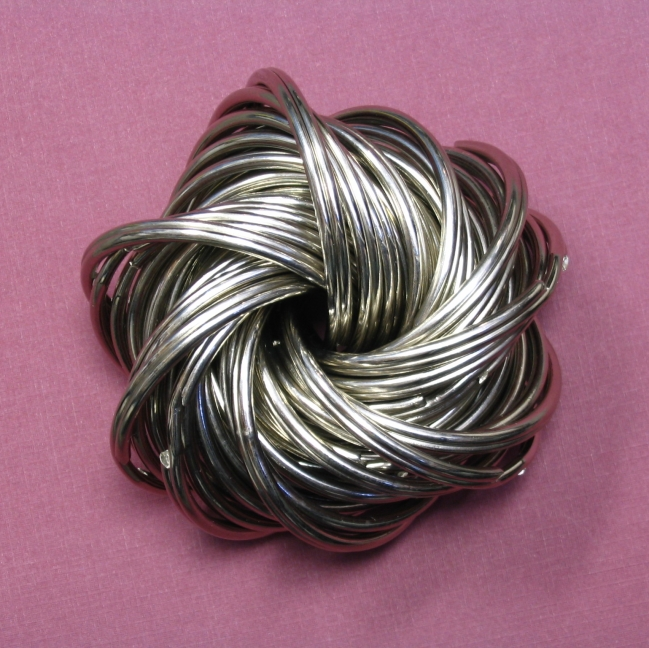
\includegraphics[width=0.8\textwidth,height=\textheight]{Hopfkeyrings.jpg}
\caption{image}
\end{figure}

\end{columns}

\end{frame}

\begin{frame}{Hopf Coordinates for SO(3) or \(S^3\)}
\protect\hypertarget{hopf-coordinates-for-so3-or-s3}{}

Similar to the Halton sequence generation on \(S^2\), we perform the
mapping:

\begin{itemize}
\item
  \(\varphi = 2\pi\cdot\mathrm{vd}(k,b_1)\) \% map to \([0,2\pi]\)
\item
  \(\psi = 2\pi\cdot\mathrm{vd}(k,b_2)\) \% map to \([0,2\pi]\) for
  SO(3), or
\item
  \(\psi = 4\pi\cdot\mathrm{vd}(k,b_2)\) \% map to \([0,4\pi]\) for
  \(S^3\)
\item
  \(z = 2\cdot\mathrm{vd}(k,b_3) - 1\) \% map to \([-1,1]\)
\item
  \(\theta = \cos^{-1}z\)
\end{itemize}

\end{frame}

\begin{frame}[fragile]{Python Code}
\protect\hypertarget{python-code}{}

\scriptsize

\begin{Shaded}
\begin{Highlighting}[]
\KeywordTok{def}\NormalTok{ sphere3_hopf(k, b):}
\NormalTok{    vd }\OperatorTok{=} \BuiltInTok{zip}\NormalTok{(vdc(k, b[}\DecValTok{0}\NormalTok{]), vdc(k, b[}\DecValTok{1}\NormalTok{]), vd(k, b[}\DecValTok{2}\NormalTok{]))}
    \ControlFlowTok{for}\NormalTok{ vd0, vd1, vd2 }\KeywordTok{in}\NormalTok{ vd:}
\NormalTok{        phi }\OperatorTok{=} \DecValTok{2}\OperatorTok{*}\NormalTok{math.pi}\OperatorTok{*}\NormalTok{vd0   }\CommentTok{# map to [0, 2*math.pi]}
\NormalTok{        psy }\OperatorTok{=} \DecValTok{4}\OperatorTok{*}\NormalTok{math.pi}\OperatorTok{*}\NormalTok{vd1   }\CommentTok{# map to [0, 4*math.pi]}
\NormalTok{        z }\OperatorTok{=} \DecValTok{2}\OperatorTok{*}\NormalTok{vd2 }\OperatorTok{-} \DecValTok{1}         \CommentTok{# map to [-1., 1.]}
\NormalTok{        theta }\OperatorTok{=}\NormalTok{ math.acos(z)}
\NormalTok{        cos_eta }\OperatorTok{=}\NormalTok{ math.cos(theta}\OperatorTok{/}\DecValTok{2}\NormalTok{)}
\NormalTok{        sin_eta }\OperatorTok{=}\NormalTok{ math.sin(theta}\OperatorTok{/}\DecValTok{2}\NormalTok{)}
\NormalTok{        s }\OperatorTok{=}\NormalTok{ [cos_eta }\OperatorTok{*}\NormalTok{ math.cos(psy}\OperatorTok{/}\DecValTok{2}\NormalTok{),}
\NormalTok{             cos_eta }\OperatorTok{*}\NormalTok{ math.sin(psy}\OperatorTok{/}\DecValTok{2}\NormalTok{),}
\NormalTok{             sin_eta }\OperatorTok{*}\NormalTok{ math.cos(phi }\OperatorTok{+}\NormalTok{ psy}\OperatorTok{/}\DecValTok{2}\NormalTok{),}
\NormalTok{             sin_eta }\OperatorTok{*}\NormalTok{ math.sin(phi }\OperatorTok{+}\NormalTok{ psy}\OperatorTok{/}\DecValTok{2}\NormalTok{)]}
        \ControlFlowTok{yield}\NormalTok{ s}
\end{Highlighting}
\end{Shaded}

\end{frame}

\begin{frame}{3-sphere}
\protect\hypertarget{sphere}{}

\begin{itemize}
\item
  Polar coordinates:

  \begin{itemize}
  \item
    \(x_0 = \cos\theta_3\)
  \item
    \(x_1 = \sin\theta_3 \cos\theta_2\)
  \item
    \(x_2 = \sin\theta_3 \sin\theta_2 \cos\theta_1\)
  \item
    \(x_3 = \sin\theta_3 \sin\theta_2 \sin\theta_1\)
  \end{itemize}
\end{itemize}

\end{frame}

\begin{frame}{n-sphere}
\protect\hypertarget{n-sphere}{}

\begin{itemize}
\item
  Polar coordinates:

  \begin{itemize}
  \item
    \(x_0 = \cos\theta_n\)
  \item
    \(x_1 = \sin\theta_n \cos\theta_{n-1}\)
  \item
    \(x_2 = \sin\theta_n \sin\theta_{n-1} \cos\theta_{n-2}\)
  \item
    \(x_3 = \sin\theta_n \sin\theta_{n-1} \sin\theta_{n-2} \cos\theta_{n-3}\)
  \item
    \(\cdots\)
  \item
    \(x_{n-1} = \sin\theta_n \sin\theta_{n-1} \sin\theta_{n-2} \cdots \cos\theta_1\)
  \item
    \(x_n = \sin\theta_n \sin\theta_{n-1} \sin\theta_{n-2} \cdots \sin\theta_1\)
  \end{itemize}
\end{itemize}

\end{frame}

\begin{frame}{How to Generate the Point Set}
\protect\hypertarget{how-to-generate-the-point-set}{}

\begin{itemize}
\item
  \(p_0 = [\cos\theta_1, \sin\theta_1]\) where
  \(\theta_1 = 2\pi\cdot\mathrm{vd}(k,b_1)\)
\item
  Let \(f_j(\theta)\) = \(\int\sin^j\theta \mathrm{d}\theta\), where
  \(\theta\in (0,\pi)\).\\
  Note: \(f_j(\theta)\) is a monotonic increasing function in
  \((0,\pi)\)
\item
  Map \(\mathrm{vd}(k,b_j)\) uniformly to \(f_j(\theta)\):\\
  \(t_j = f_j(0) + (f_j(\pi) - f_j(0)) \mathrm{vd}(k,b_j)\)
\item
  Let \(\theta_j = f_j^{-1}(t_j)\)
\item
  Define \(p_n\) recursively as:\\
  \(p_n = [\cos\theta_n, \sin\theta_n \cdot p_{n-1}]\)
\end{itemize}

\end{frame}

\begin{frame}{\(S^3\) projected on four different spheres}
\protect\hypertarget{s3-projected-on-four-different-spheres}{}

\begin{figure}
\centering
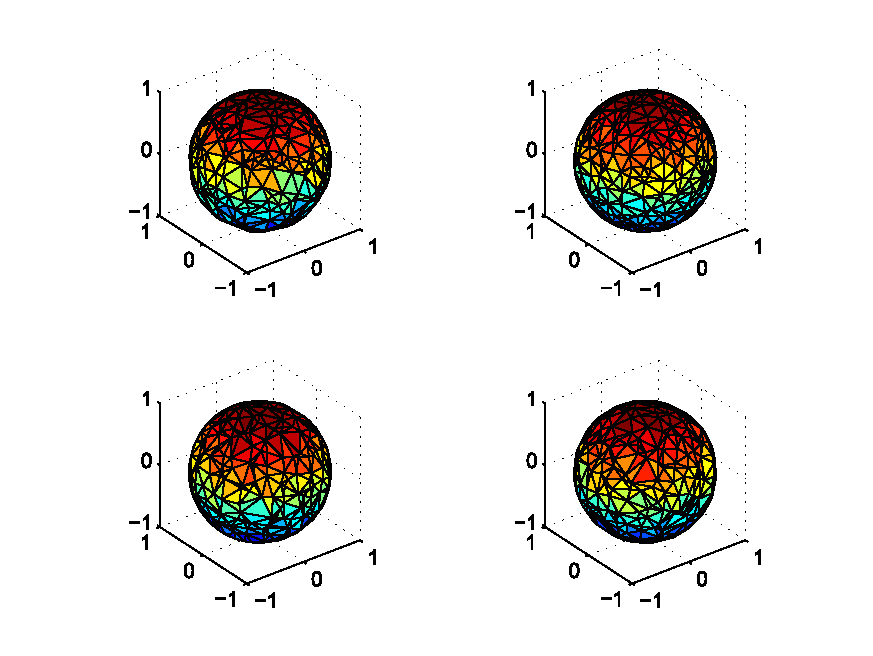
\includegraphics[width=0.9\textwidth,height=\textheight]{res_proj.pdf}
\caption{image}
\end{figure}

\end{frame}

\hypertarget{numerical-experiments}{%
\section{Numerical Experiments}\label{numerical-experiments}}

\begin{frame}{Testing the Correctness}
\protect\hypertarget{testing-the-correctness}{}

\begin{itemize}
\item
  Compare the dispersion with the random point-set

  \begin{itemize}
  \item
    Construct the convex hull for each point-set
  \item
    Dispersion roughly measured by the difference of the maximum
    distance and the minimum distance between every two neighbour
    points: \[\max_{a \in \mathcal{N}(b)} \{D(a,b)\} - 
            \min_{a \in \mathcal{N}(b)} \{ D(a, b) \}\] where
    \(D(a,b) = \sqrt{1 - a^\top b}\)
  \end{itemize}
\end{itemize}

\end{frame}

\begin{frame}{Random sequences}
\protect\hypertarget{random-sequences}{}

\begin{itemize}
\item
  To generate random points on \(S^n\), spherical symmetry of the
  multidimensional Gaussian density function can be exploited.
\item
  Then the normalized vector (\(x_i/\|x_i\|\)) is uniformly distributed
  over the hypersphere \(S^n\). {[}Fishman, G. F. (1996){]}
\end{itemize}

\end{frame}

\begin{frame}{Convex Hull with \(\approx 400\) points}
\protect\hypertarget{convex-hull-with-approx-400-points}{}

\begin{figure}
\centering
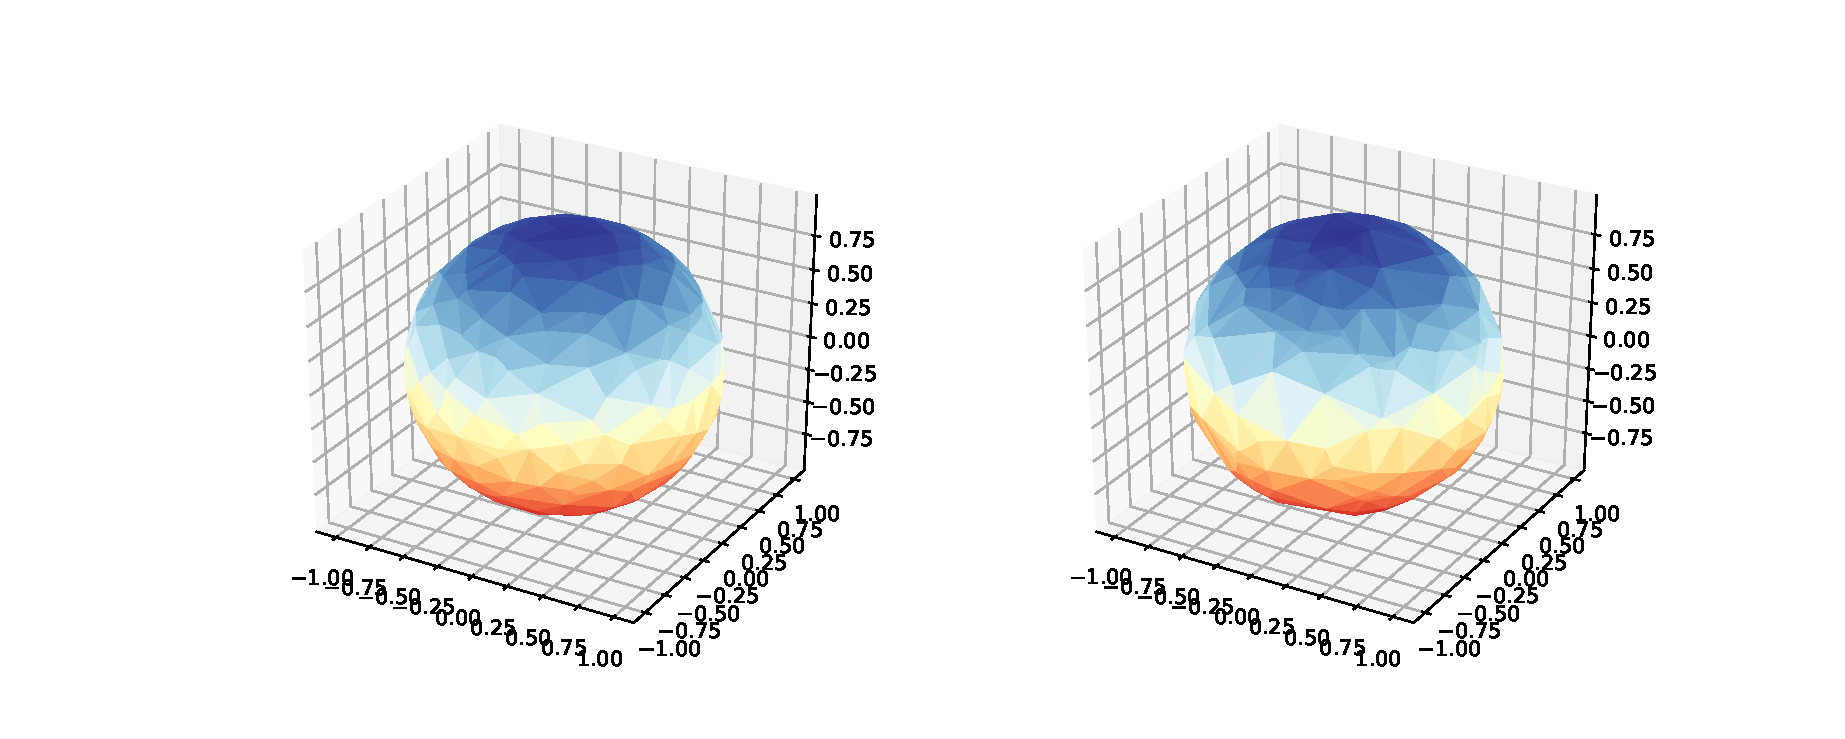
\includegraphics[width=0.9\textwidth,height=\textheight]{res_compare.pdf}
\caption{image}
\end{figure}

Left: our, right: random

\end{frame}

\begin{frame}{Result for \(S^3\)}
\protect\hypertarget{result-for-s3}{}

\begin{figure}
\centering
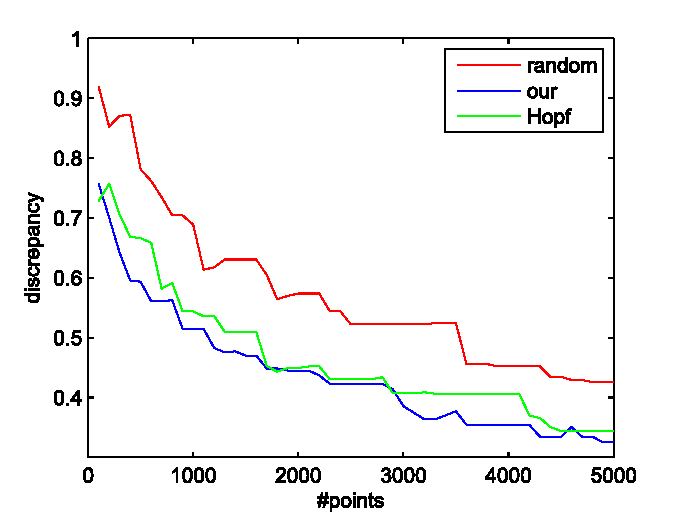
\includegraphics[width=0.9\textwidth,height=\textheight]{res_hopf.pdf}
\caption{image}
\end{figure}

\end{frame}

\begin{frame}{Result for \(S^4\)}
\protect\hypertarget{result-for-s4}{}

\begin{figure}
\centering
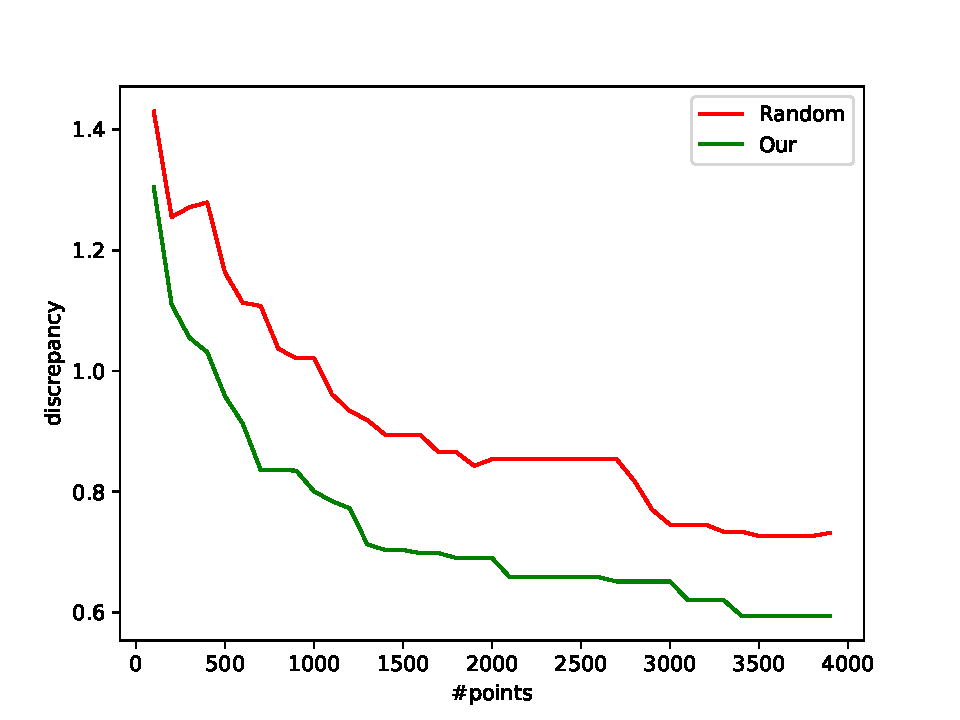
\includegraphics[width=0.9\textwidth,height=\textheight]{res_S4.pdf}
\caption{image}
\end{figure}

\end{frame}

\hypertarget{conclusions}{%
\section{Conclusions}\label{conclusions}}

\begin{frame}{Conclusions}
\protect\hypertarget{conclusions-1}{}

\begin{itemize}
\item
  Proposed method generates low-discrepancy point-set in nearly linear
  time
\item
  The result outperforms the corresponding random point-set, especially
  when the number of points is small
\item
  The MATLAB source code is available in public (or upon request)
\end{itemize}

\end{frame}

\begin{frame}[allowframebreaks]{References}
\protect\hypertarget{references}{}

\hypertarget{refs}{}
\leavevmode\hypertarget{ref-cui1997equidistribution}{}%
Cui, Jianjun, and Willi Freeden. 1997. “Equidistribution on the Sphere.”
\emph{SIAM Journal on Scientific Computing} 18 (2). SIAM:595–609.

\leavevmode\hypertarget{ref-mandic2011filter}{}%
Mandic, DP, and others. 2011. “Filter Bank Property of Multivariate
Empirical Mode Decomposition.” \emph{Signal Processing, IEEE
Transactions on} 59 (5). IEEE:2421–6.

\leavevmode\hypertarget{ref-rehman2010multivariate}{}%
Rehman, Naveed, and Danilo P Mandic. 2010. “Multivariate Empirical Mode
Decomposition.” \emph{Proceedings of the Royal Society A: Mathematical,
Physical and Engineering Science} 466 (2117). The Royal
Society:1291–1302.

\leavevmode\hypertarget{ref-utkovski2006construction}{}%
Utkovski, Zoran, and Juergen Lindner. 2006. “On the Construction of
Non-Coherent Space Time Codes from High-Dimensional Spherical Codes.” In
\emph{Spread Spectrum Techniques and Applications, 2006 Ieee Ninth
International Symposium on}, 327–31. IEEE.

\leavevmode\hypertarget{ref-wong1997sampling}{}%
Wong, Tien-Tsin, Wai-Shing Luk, and Pheng-Ann Heng. 1997. “Sampling with
Hammersley and Halton Points.” \emph{Journal of Graphics Tools} 2 (2).
Taylor \& Francis:9–24.

\leavevmode\hypertarget{ref-yershova2010generating}{}%
Yershova, Anna, Swati Jain, Steven M LaValle, and Julie C Mitchell.
2010. “Generating Uniform Incremental Grids on so (3) Using the Hopf
Fibration.” \emph{The International Journal of Robotics Research} 29
(7). SAGE Publications:801–12.

\end{frame}

\end{document}
